%!TeX program = pdflatex
% Zixing Jiang's Curriculum Vitae
% Email: zxjiang@surgery.cuhk.edu.hk
% Web: https://zixingjiang.com/
% Repo: https://github.com/zixingjiang/cv

\documentclass[11pt,letterpaper]{report}

\usepackage[T1]{fontenc} % output T1 font encoding (8-bit) for accented characters as single glyph
\usepackage[strict,autostyle]{csquotes} % smart and nestable quote marks
\usepackage[USenglish]{babel} % regionalize hyphens, quote marks, etc automatically
\usepackage{microtype}% improve text appearance with kerning, etc
\usepackage{datetime} % enable formatting of date output
\usepackage{tabto}    % make nice tabbing
\usepackage{setspace} % custom line spacing (should load this before hyperref)
\usepackage{hyperref} % enable hyperlinks and pdf metadata
\usepackage{geometry} % manually set page margins
\usepackage{enumitem} % enumerate with [resume] option
\usepackage{titlesec} % allow custom section fonts
\usepackage[dvipsnames]{xcolor}
\usepackage[fixed]{fontawesome5}
\usepackage{textcase}
\usepackage{graphicx}
\usepackage[export]{adjustbox}

% what is your name?
\newcommand{\myname}{JIANG Zixing}

% select default typefaces
\usepackage{ebgaramond} % document's serif font
\usepackage{tgheros}  % document's sans serif font

% how far to tab for list items with left-aligned date: different fonts need different widths
\newcommand{\listtabwidth}{1.7cm}

% define font to use as document's title
\newcommand{\namefont}[1]{{\normalfont\bfseries\Huge{#1}}}

% set section heading fonts and before/after spacing
\SetTracking{encoding=*, family=\sfdefault}{30} % increase sans serif headings tracking
\titleformat{\section}{\lsstyle\sffamily\small\bfseries\MakeUppercase}{}{}{}{}
\titlespacing{\section}{0pt}{30pt plus 4pt minus 4pt}{8pt plus 2pt minus 2pt}

% set subsection heading fonts and before/after spacing
\titleformat{\subsection}{\lsstyle\sffamily\footnotesize\bfseries}{}{}{}{}
\titlespacing{\subsection}{0pt}{16pt plus 4pt minus 4pt}{4pt plus 2pt minus 2pt}

% set page margins (assumes letter paper)
\geometry{
  left=1.0in,
  right=1.0in,
  top=0.8in,
  bottom=1.2in
}

% prevent paragraph indentation
\setlength\parindent{0em}

% set line spacing
\setstretch{0.9}

% define space between list items
\newcommand{\listitemspace}{0.25em}

% make unordered lists without bullets and use compact spacing
\renewenvironment{itemize}
{\begin{list}{}{\setlength{\leftmargin}{0em}
			\setlength{\parskip}{0em}
			\setlength{\itemsep}{\listitemspace}
			\setlength{\parsep}{\listitemspace}}}
	{\end{list}}

% make tabbed lists so content is left-aligned next to years
\TabPositions{\listtabwidth}
\newlist{tablist}{description}{3}
\setlist[tablist]{leftmargin=\listtabwidth,
	labelindent=0em,
	topsep=0em,
	partopsep=0em,
	itemsep=\listitemspace,
	parsep=\listitemspace,
	font=\normalfont}

% print only the month and year when using \today
\newdateformat{monthyeardate}{\monthname[\THEMONTH] \THEYEAR}

% define hyperlink appearance and metadata for pdf properties
\hypersetup{
	colorlinks  = true,
	urlcolor    = Blue,
	citecolor   = blue,
	linkcolor   = Blue,
	pdfauthor   = {\myname},
	pdftitle    = {\myname: Curriculum Vitae},
	pdfsubject  = {Curriculum Vitae},
	pdfpagemode = UseNone
}


\usepackage[multiple, hang, flushmargin, stable]{footmisc}
\usepackage{fnpct}
\addtolength{\skip\footins}{1.5pc plus 5pt}
\renewcommand\thefootnote{\textcolor{Blue}{\arabic{footnote}}}


\usepackage{fancyhdr}
\usepackage{lastpage}

% Custom footer for the first page
\fancypagestyle{firstpagefooter}{
	\fancyhf{}
	%\fancyfoot[R]{\monthyeardate\today}
	\fancyfoot[C]{\thepage ~of \pageref{LastPage}}
	\renewcommand{\headrulewidth}{0pt}
	\renewcommand{\footrulewidth}{0pt}
}

% Custom footer for the rest of the pages
\pagestyle{fancy}
\fancyhf{}
\fancyfoot[C]{\thepage ~of \pageref{LastPage}}
\renewcommand{\headrulewidth}{0pt}

\begin{document}
	\thispagestyle{firstpagefooter}
	\raggedright{}
	
% display your name as the document title
\namefont{\myname}
	
% affiliation and contact info blocks
\vspace{1em}
\begin{minipage}[t]{0.700\textwidth}
	Department of Surgery\\ 
	Faculty of Medicine\\
	The Chinese University of Hong Kong (CUHK)
\end{minipage}
\hfil
\begin{minipage}[t]{0.295\textwidth}
	% contact info details, right-aligned
	\flushright{}
	\href{mailto:zxjiang@surgery.cuhk.edu.hk}{zxjiang@surgery.cuhk.edu.hk} \\
	+852 5954 9660 \\
	\href{https://zixingjiang.com}{https://zixingjiang.com}\\
\end{minipage}
	
	\section*{Education}
\begin{tablist}
	\item[M.Phil.]  \tab{}Surgery, CUHK, In progress 2024-- \\
	Research Topic: Robotic Ultrasound Imaging and Ultrasound-Guided Biopsy, supervised by \href{https://www.surgery.cuhk.edu.hk/profile.asp?alias=zli}{Prof. LI Zheng}
	\item[B.Eng.]  \tab{}Electronic Information Engineering, \textit{First-Class Honors}, CUHK-Shenzhen, 2023\\
	Final Year Project: Control of the Multi-Joint Manipulator for Grasping on Water Surface, supervised by \href{https://sse.cuhk.edu.cn/en/faculty/qianhuihuan}{Prof. QIAN Huihuan}
\end{tablist}



\section*{Professional Experience}
\begin{tablist}
	\item[2023--24]   \tab{}Advanced Bio-Medical Robotics Laboratory (ABML), CUHK \\
	Research Assistant, Robotic Ultrasound Project
	
	\item[2020--23]   \tab{}Robotics \& Artificial Intelligence Laboratory (RAIL), CUHK-Shenzhen \\
	Research Intern, Medical Robotics Group, 2023.02--08\\
	Research Intern, Marine Robotics Group, 2020.09--2023.02
\end{tablist}
\section*{Research Interests}
\begin{itemize}
	\item Robotics: Calibration, Perception, Motion Planning \& Control
	\item Medical Robotics: Image-Guided Robotic Interventions, Robot-Assisted Imaging
\end{itemize}

\section*{Selected Projects}
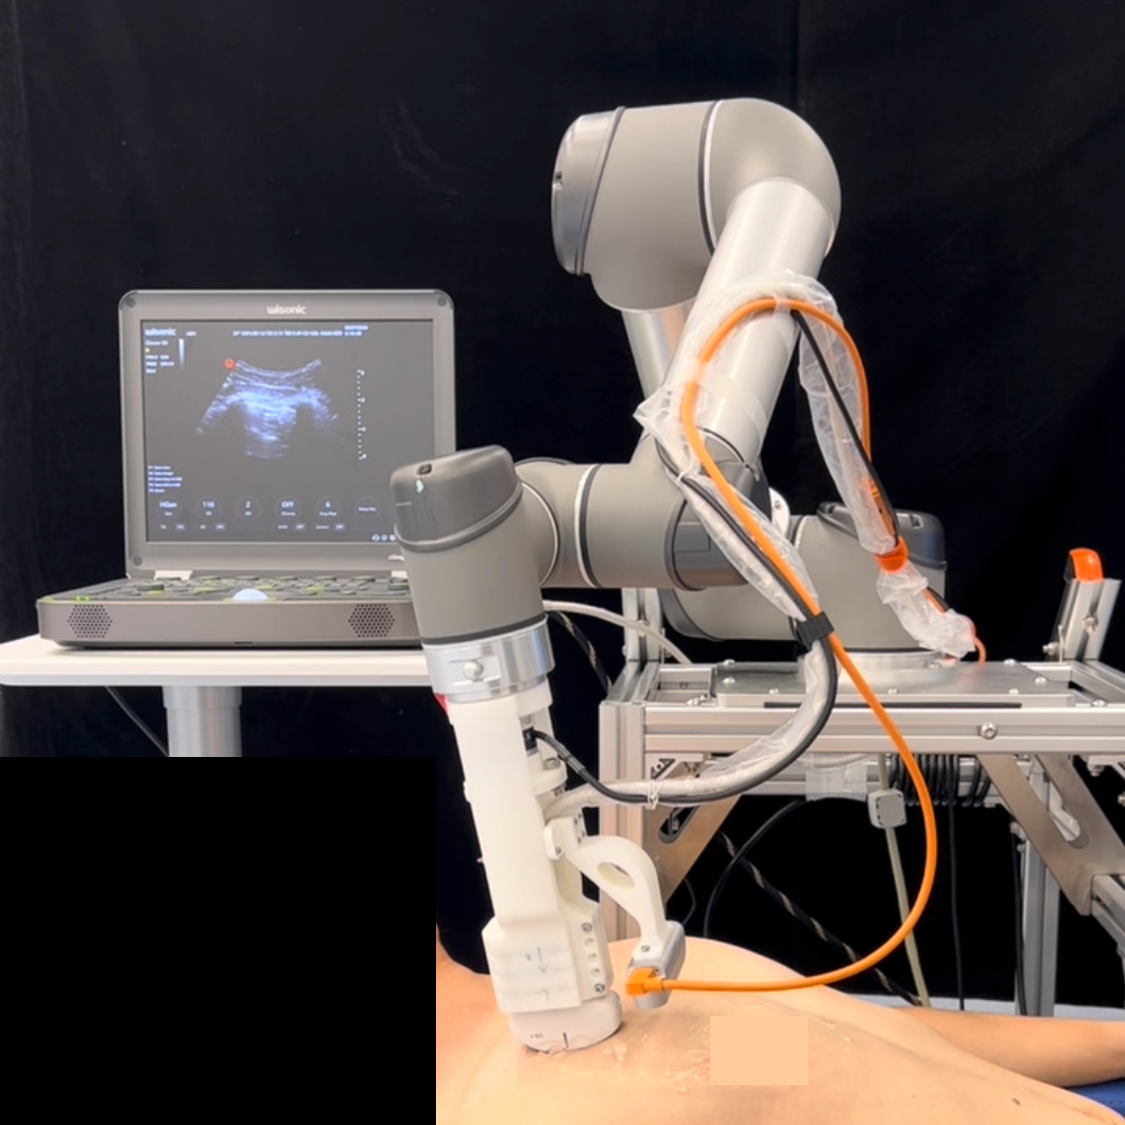
\includegraphics[width=0.22\linewidth, valign=T]{img/usrobot}\hfill
\begin{minipage}[t]{0.75\linewidth}
	\vspace{0pt}\par
\begin{itemize}
	\item Robotic Ultrasound Imaging\\ABML, CUHK, 2023--
	\item Participating in a research project aimed at developing a robotic system for teleoperated and autonomous ultrasound examinations.
	\item My contributions: system integration; development of core algorithms including visual servoing, force control, motion planning, teleoperation, etc; assistance in conducting preclinical validation for lung ultrasound applications.
\end{itemize}
\end{minipage}\\~\\

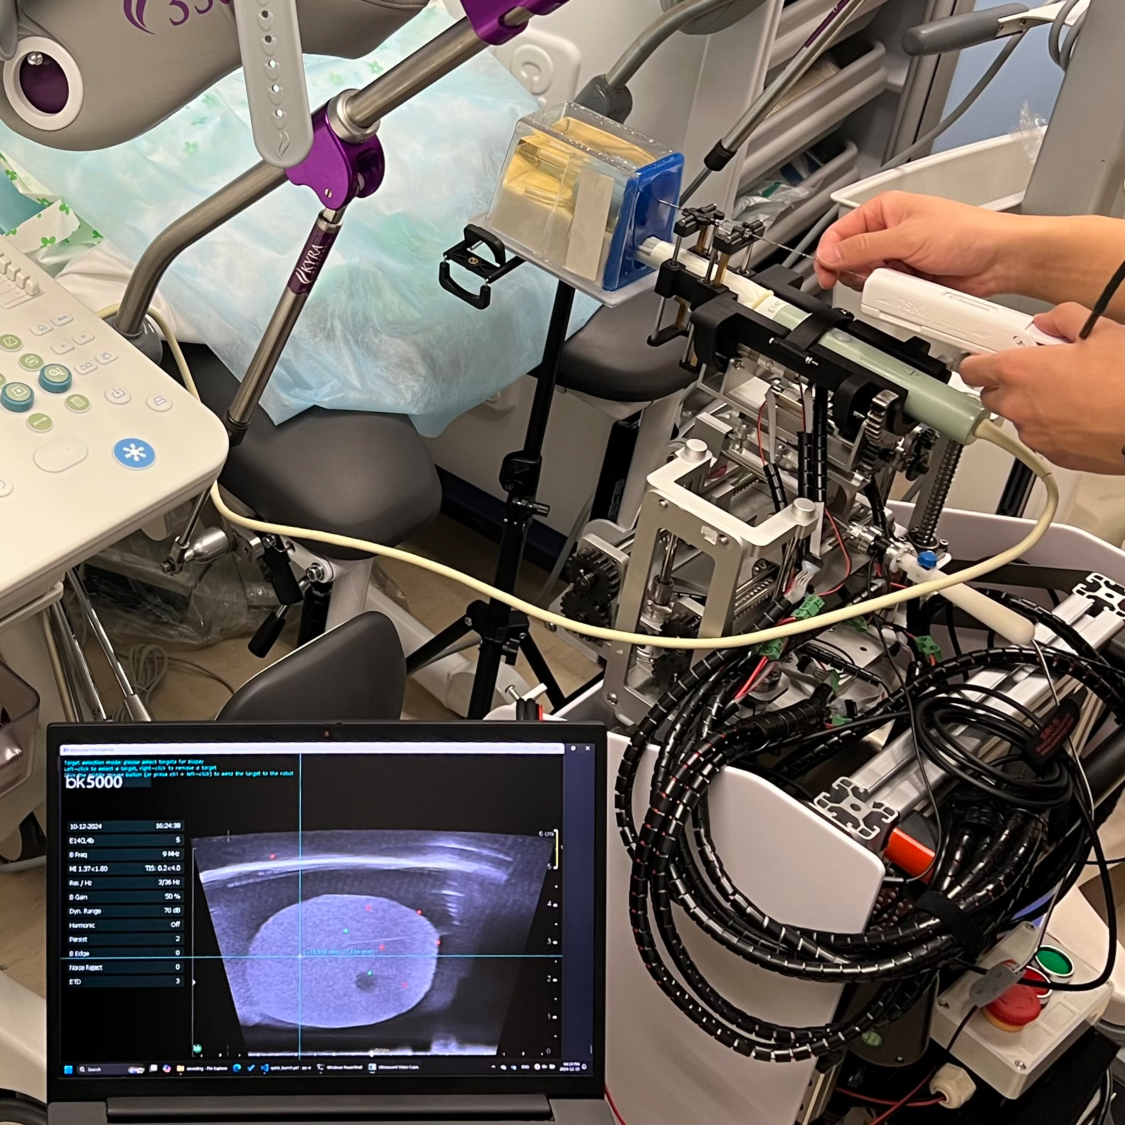
\includegraphics[width=0.22\linewidth, valign=T]{img/prostate-biopsy}\hfill
\begin{minipage}[t]{0.75\linewidth}
	\vspace{0pt}\par
	\begin{itemize}
		\item Robot-Assisted Prostate Biopsy\\ABML, CUHK, 2024--
		\item Participating in a research project aimed at developing an assistive navigation robot for ultrasound-guided transperineal prostate biopsy.
		\item My contributions: development of navigation and visualization interface; assistance in conducting clinical trials. 
	\end{itemize}
\end{minipage}\\~\\

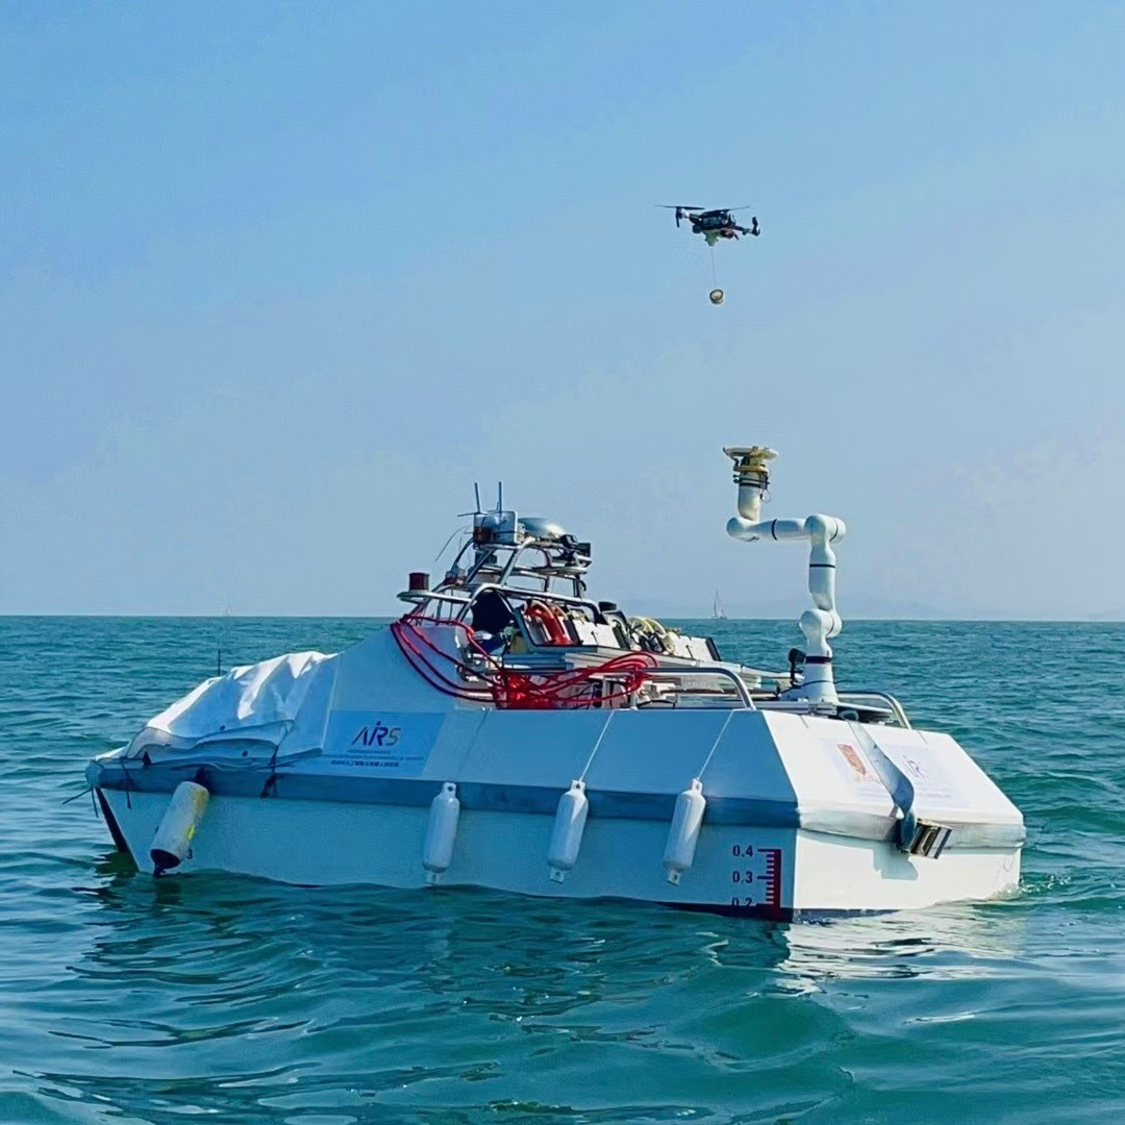
\includegraphics[width=0.22\linewidth, valign=T]{img/usv-uav}\hfill
\begin{minipage}[t]{0.75\linewidth}
	\vspace{0pt}\par
	\begin{itemize}
			\item USV-UAV Cooperative System\\RAIL, CUHK-Shenzhen, 2020--23
			\item Engaged in a research project aimed at developing an unmanned surface vehicle (USV) as a carrier for unmanned aerial vehicles (UAVs) for marine applications.
			\item My contributions: assistance in developing manipulator-assisted UAV launch and recovery solutions, including end-effector design and motion planning algorithms.
		\end{itemize}
\end{minipage}

\section*{Publications}
\subsection*{Journal Articles}
\begin{tablist}
	\item[2025]	 \tab{}L. Lei$^*$, Y. Hu$^*$, \textbf{Z. Jiang}$^*$, J. Miao, X. Luo, Y. Zhang, Q. Wang, S. Wang, Z. Li, and P.-A. Heng, ``Towards Lung Ultrasound Automation: Fully Automonous Robotic Longitudinal and Transverse Scans Along Intercostal Spaces,'' \textit{IEEE Transactions on Medical Robotics and Bionics}, vol. 7, no. 2, pp. 768--781, doi: \href{https://doi.org/10.1109/TMRB.2025.3550663}{10.1109/TMRB.2025.3550663} ($^*$ indicates co-first authors).
	
	\item[2024]  \tab{}R. Xu, \textbf{Z. Jiang}, B. Liu, Y. Wang, and H. Qian, ``Confidence-Aware Object Capture for a Manipulator Subject to Floating-Base Disturbances,'' \textit{IEEE Transactions on Robotics}, vol. 40, pp. 4396--4413, doi: \href{https://doi.org/10.1109/TRO.2024.3463476}{10.1109/TRO.2024.3463476}.
\end{tablist}
	
\subsection*{Conference Proceedings}
\begin{tablist}
	\item[2025] \tab X. Luo, \textbf{Z. Jiang}, M. C. Lei, Y. Xian, Y. Hu, A. Dong, P. K. F. Chiu, Y.-H. Liu, and Z. Li, ``Design and Geometry-Aware Planning of a Novel Probe-Scanning Manipulator with RCM Constraint,'' \textit{2025 IEEE/RSJ International Conference on Intelligent Robots and Systems,} Hangzhou, China, in press (\textcolor{magenta}{Best Paper Award Finalist}).
	
	\item[2023]   \tab{}Y. Jiang, R. Xu, \textbf{Z. Jiang} and H. Qian, ``Design, Modeling and Control of A Novel USV-Manipulator System,'' \textit{2023 IEEE International Conference on Real-time Computing and Robotics}, Datong, China, pp. 206-211, doi: \href{https://doi.org/10.1109/RCAR58764.2023.10249802}{ 10.1109/RCAR58764.2023.10249802}.
		
	\item[2022]   \tab{}C. Liu, \textbf{Z. Jiang}, R. Xu, X. Ji, L. Zhang and H. Qian, ``Design and Optimization of a Magnetic Catcher for UAV Landing on Disturbed Aquatic Surface Platforms,'' \textit{2022 International Conference on Robotics and Automation}, Philadelphia, PA, USA, pp. 1162-1168, doi: \href{https://doi.org/10.1109/ICRA46639.2022.9812270}{ 10.1109/ICRA46639.2022.9812270}.
\end{tablist}

\subsection*{Patents}
\begin{tablist}	
	\item[2024]   \tab{}C. Liu, Z. Cao, \textbf{Z. Jiang}, R. Xu, X. Ji, and H. Qian, \textit{Unmanned Aerial Vehicle Landing System, Landing Method and Storage Medium}, Chinese patent \href{https://patents.google.com/patent/CN115167522B/en?oq=CN115167522B}{CN115167522B}.	
	
	\item[2023]   \tab{}\textbf{Z. Jiang}, X. Ji, C. Liu, and H. Qian, \textit{Four-wing Flapping Wing Micro Water Surface Aircraft and Flight Method}, Chinese patent \href{https://patents.google.com/patent/CN114889821B/en?oq=CN114889821B}{CN114889821B}.
	
	\item[2022]   \tab{}X. Ji, Z. Song, \textbf{Z. Jiang}, and H. Qian, \textit{Flapping Wing Mechanism and Miniature Water Surface Flapping Wing Aircraft}, Chinese patent \href{https://patents.google.com/patent/CN217320745U/en?oq=CN217320745U}{CN217320745U}.  
	
	\item[2022]   \tab{}X. Ji, Z. Song, \textbf{Z. Jiang}, and H. Qian, \textit{Flapping Wing Mechanism based on Double Cranks and Micro Water Surface Flapping Wing Aircraft}, Chinese patent \href{https://patents.google.com/patent/CN217320744U/en?oq=CN217320744U}{CN217320744U}.  
\end{tablist}

\section*{Conference Activity}
\subsection*{Conference Presentation}
Presenting author \textit{italicized} if other than first author.\vspace{1ex}\\
\begin{tablist}	
	\item[2024] \tab \textbf{Z. Jiang}, Y. Hu, X. Luo, J. Miao, Y. Zhang, L. Lei, S. Wang, P.-A. Heng, and Z. Li, ``A Collaborative Robotic System with In-Plane Orientation Adjustment for Lung Ultrasonography,'' presented at workshop \textit{Autonomy in Robotic Surgery: State of the art, technical and regulatory challenges for clinical application}, ICRA 2024, Yokohama, Japan, May 13.
\end{tablist}
	
		
\section*{Awards and Honors}
\begin{tablist}	
	\item[2025] \tab Prof. Charles K. Kao Student Creativity Awards, CUHK\\
	Finalist, Team: \textit{A Novel Robotic System for Minimally Invasive Transperineal Prostate Biopsy with Enhanced Safety.}
	
	\item[2024] \tab The 14th ``Challenge Cup'' Qin Chuang Yuan National College Students' Entrepreneurship Competition, China\\
	Bronze Award, Team: \textit{ColoMAG: A Magnet-Assisted System for Colorectal Cancer Screening and Early Surgical Treatment.}	

	\item[2023]   \tab School of Science and Engineering Academic Year 2022--23 Dean's List Award, CUHK-Shenzhen
	
	\item[2021--22]   \tab The 17--19th rounds of  Undergraduate Research Award, CUHK-Shenzhen\\
	Project: \textit{Bio-Inspired Robot for Aquatic-Aerial Hybrid Locomotion.}
	
	\item[2020] \tab RoboCom Robot Developer Competition (southern China regional)\\
	{Second Prize, semi-autonomous palletizing competition};\\
	{Third Prize, semi-autonomous palletizing time trial};\\
	{Third Prize, autonomous palletizing competition};\\
	\textit{CUHK-Shenzhen representative team}.
\end{tablist}

\section*{Extracurricular Activity}
\begin{tablist}
	\item[2020--22]   \tab President, Student Robotics Association, CUHK-Shenzhen 
\end{tablist}

\section*{Service}
\subsection*{Academic Journal Peer Review}
\begin{itemize}
	\item \textit{IEEE Robotics and Automation Letters}
\end{itemize}
\subsection*{Conference Peer Review}
\begin{itemize}
	\item \textit{IEEE International Conference on Robotics and Automation}
	\item \textit{IEEE/RSJ International Conference	on Intelligent Robots and Systems}
	\item \textit{IEEE International Conference on Robotics and Biomimetics}
\end{itemize}


\section*{Course Taught}
\begin{itemize}
	\item BMEG5750 Medical Robotics, CUHK (Teaching Assistant)
\end{itemize}

\section*{Open Source Contributions}
\subsection*{Maintainer}
\begin{itemize}
	\item  \href{https://github.com/zixingjiang/minimal_handeye_ros2}{minimal\_handeye\_ros2}\faGithub: A minimal ROS2 node for calculating the hand-eye calibration problem.
	\item  \href{https://github.com/zixingjiang/ndi_ros2_driver}{ndi\_ros2\_driver}\faGithub: ROS2-control integration for Northern Digital Inc. (NDI) electromagnetic tracking and optical navigation systems.
\end{itemize}
\subsection*{Contributor}
\begin{itemize}
	\item \href{https://github.com/fzi-forschungszentrum-informatik/cartesian_controllers}{cartesian\_controllers}\faGithub: A set of Cartesian controllers for the ROS1 and ROS2-control framework.
	\item \href{https://github.com/PlusToolkit}{PLUS (Public software Library for UltraSound) Toolkit}\faGithub: Open-source toolkit for data acquisition, pre-processing, and calibration for navigated image-guided interventions.
\end{itemize}

\section*{Skills}
\begin{itemize}
	\item {Programming Languages:} Python, C++, C, MATLAB
	\item {Software:} ROS, SolidWorks, OpenCV, Open3D, MuJoCo, SOFA, 3D Slicer, \LaTeX, and more
	\item {Hardware:} Experience with robotic arms (Universal Robots UR5, Franka Emika Panda, Interbotix WidowX-250), microcontrollers (Arduino, STM32, ESP32), single-board computers (Raspberry Pi), and diverse sensors (RGB-D cameras, ultrasound, optical, force/torque, haptic, magnetic field, etc.)
	\item {Languages:} Chinese (native), English (fluent)
\end{itemize}

%\newpage
\section*{References}
\begin{itemize}
	\item \textbf{Prof. LI Zheng} ~{\scriptsize \faEnvelope}\href{mailto:zhengli@cuhk.edu.hk}{zhengli@cuhk.edu.hk}\\
	Professor\\
	Department of Surgery\\
	The Chinese University of Hong Kong
	
	{M.Phil. Supervisor}

	\vspace{1ex}
	
	\item \textbf{Prof. QIAN Huihuan (Alex)} ~{\scriptsize \faEnvelope}\href{mailto:hhqian@cuhk.edu.cn}{hhqian@cuhk.edu.cn}\\
	Associate Professor\\School of Science and Engineering\\The Chinese University of Hong Kong, Shenzhen

	{B.Eng. Final Year Project Supervisor}

\end{itemize}
	
% display today's date as Month Year after a vertical space below the end of the text
\begin{center}
	\vfill
	Last update: \monthyeardate\today
\end{center}
	
\end{document}